\documentclass{beamer}
\usepackage[utf8]{inputenc}

\usetheme{Madrid}
\usecolortheme{default}
\usepackage{amsmath,amssymb,amsfonts,amsthm}
\usepackage{txfonts}
\usepackage{tkz-euclide}
\usepackage{listings}
\usepackage{adjustbox}
\usepackage{array}
\usepackage{tabularx}
\usepackage{gvv}
\usepackage{lmodern}
\usepackage{circuitikz}
\usepackage{tikz}
\usepackage{graphicx}

\setbeamertemplate{page number in head/foot}[totalframenumber]

\usepackage{tcolorbox}
\tcbuselibrary{minted,breakable,xparse,skins}



\definecolor{bg}{gray}{0.95}
\DeclareTCBListing{mintedbox}{O{}m!O{}}{%
  breakable=true,
  listing engine=minted,
  listing only,
  minted language=#2,
  minted style=default,
  minted options={%
    linenos,
    gobble=0,
    breaklines=true,
    breakafter=,,
    fontsize=\small,
    numbersep=8pt,
    #1},
  boxsep=0pt,
  left skip=0pt,
  right skip=0pt,
  left=25pt,
  right=0pt,
  top=3pt,
  bottom=3pt,
  arc=5pt,
  leftrule=0pt,
  rightrule=0pt,
  bottomrule=2pt,
  toprule=2pt,
  colback=bg,
  colframe=orange!70,
  enhanced,
  overlay={%
    \begin{tcbclipinterior}
    \fill[orange!20!white] (frame.south west) rectangle ([xshift=20pt]frame.north west);
    \end{tcbclipinterior}},
  #3,
}
\lstset{
    language=C,
    basicstyle=\ttfamily\small,
    keywordstyle=\color{blue},
    stringstyle=\color{orange},
    commentstyle=\color{green!60!black},
    numbers=left,
    numberstyle=\tiny\color{gray},
    breaklines=true,
    showstringspaces=false,
}
%------------------------------------------------------------
%This block of code defines the information to appear in the
%Title page
\title %optional
{1.11.15}
%\subtitle{A short story}

\author % (optional)
{Gautham-AI25BTECH11013}



\begin{document}


\frame{\titlepage}
\begin{frame}{Question}
Write the direction ratios of the vector 3$\Vec{a}+2\Vec{b}$ where $\Vec{a}=\overrightarrow{i}+\overrightarrow{j}-2\overrightarrow{k}$ and $\Vec{b}=2\overrightarrow{i}-4\overrightarrow{j}+5\overrightarrow{k}$.
\end{frame}
\begin{frame}{Theoretical Solution}
The given vectors $\Vec{a}$ and $\Vec{b}$ are 
\begin{align}
\Vec{a}=\myvec{1 \\ 1 \\ -2} \\
\Vec{b}=\myvec{2 \\ -4 \\ 5}
\end{align}
The direction ratios of the vector $3\Vec{a}+2\Vec{b}$ are
\end{frame}
\begin{frame}{Theoretical Solution}
\begin{align}
  3\Vec{a}+2\Vec{b}=\myvec{a&b}\myvec{3 \\ 2}\\
  3\Vec{a}+2\Vec{b}=\myvec{1 & 2 \\ 1 &-4 \\ -2 & 5}\myvec{3\\2}\\
  3\Vec{a}+2\Vec{b}=\myvec{3(1)+2(2)\\3(1)+2(-4)\\3(-2)+2(5)}\\
  3\Vec{a}+2\Vec{b}=\myvec{7\\-5\\4}
\end{align}
\end{frame}

\begin{frame}[fragile]
\frametitle{C Function}
   \begin{lstlisting}
#include <stdio.h>

// Function to compute 3a + 2b and return direction ratios
void compute_vector_sum(double a_i, double a_j, double a_k, 
                       double b_i, double b_j, double b_k,
                       double *result_i, double *result_j, double *result_k) {
    // Calculate 3a + 2b
    *result_i = 3 * a_i + 2 * b_i;
    *result_j = 3 * a_j + 2 * b_j;
    *result_k = 3 * a_k + 2 * b_k;
}

// Function to print vector components
void print_vector(const char *name, double i, double j, double k) {
    printf("%s = %.1fi + %.1fj + %.1fk\n", name, i, j, k);
}
   \end{lstlisting}
\end{frame}
\begin{frame}[fragile]
\frametitle{Main C Code}
   \begin{lstlisting}
 #include <stdio.h>

// Function declarations
void compute_vector_sum(double a_i, double a_j, double a_k, 
                       double b_i, double b_j, double b_k,
                       double *result_i, double *result_j, double *result_k);
void print_vector(const char *name, double i, double j, double k);
int main() {
    // Given vectors
    double a_i = 1.0, a_j = 1.0, a_k = -2.0;  // a = i + j - 2k
    double b_i = 2.0, b_j = -4.0, b_k = 5.0;  // b = 2i - 4j + 5k
    
    // Result vector
    double result_i, result_j, result_k;
   \end{lstlisting}
\end{frame}
\begin{frame}[fragile]
\frametitle{Main C Code}
   \begin{lstlisting}
  
    // Compute 3a + 2b
    compute_vector_sum(a_i, a_j, a_k, b_i, b_j, b_k, 
                      &result_i, &result_j, &result_k);
    
    // Print results
    printf("Vector Operations:\n");
    printf("==================\n");
    print_vector("a", a_i, a_j, a_k);
    print_vector("b", b_i, b_j, b_k);
    print_vector("3a + 2b", result_i, result_j, result_k);
    
    printf("\nDirection ratios of 3a + 2b:\n");
    printf("x-component: %.1f\n", result_i);
    printf("y-component: %.1f\n", result_j);
    printf("z-component: %.1f\n", result_k);
    return 0;
}
   \end{lstlisting}
\end{frame}
\begin{frame}[fragile]
\frametitle{Python Code}
   \begin{lstlisting}
from ctypes import CDLL, c_double, POINTER
import matplotlib.pyplot as plt
import numpy as np
from mpl_toolkits.mplot3d import Axes3D

lib = CDLL('./libvector.so')
lib.compute_vector_sum.argtypes = [
    c_double, c_double, c_double,  # a components
    c_double, c_double, c_double,  # b components
    POINTER(c_double), POINTER(c_double), POINTER(c_double)  # result components
]
lib.compute_vector_sum.restype = None
a = [1.0, 1.0, -2.0]  # i + j - 2k
b = [2.0, -4.0, 5.0]  # 2i - 4j + 5k
result_i = c_double()
result_j = c_double()
result_k = c_double()
   \end{lstlisting}
\end{frame}
\begin{frame}[fragile]
\frametitle{Python Code}
   \begin{lstlisting}
# Call the C function
lib.compute_vector_sum(
    c_double(a[0]), c_double(a[1]), c_double(a[2]),
    c_double(b[0]), c_double(b[1]), c_double(b[2]),
    result_i, result_j, result_k
)
result_vector = [result_i.value, result_j.value, result_k.value]
print("Vector Operations using Python and C Library")
print("===========================================")
print(f"Vector a = {a[0]}i + {a[1]}j + {a[2]}k")
print(f"Vector b = {b[0]}i + {b[1]}j + {b[2]}k")
print(f"3a + 2b = {result_vector[0]:.1f}i + {result_vector[1]:.1f}j + {result_vector[2]:.1f}k")
print(f"\nDirection ratios of 3a + 2b:")
print(f"x-component: {result_vector[0]:.1f}")
print(f"y-component: {result_vector[1]:.1f}")
print(f"z-component: {result_vector[2]:.1f}")
\end{lstlisting}
\end{frame}
\begin{frame}[fragile]
\frametitle{Python Code}
   \begin{lstlisting}
# Create a detailed 3D plot
fig = plt.figure(figsize=(14, 10))
ax = fig.add_subplot(111, projection='3d')
origin = [0, 0, 0]
ax.quiver(*origin, *a, color='red', arrow_length_ratio=0.1, linewidth=3, 
          label=f'a = {a[0]}i + {a[1]}j + {a[2]}k')
ax.quiver(*origin, *b, color='blue', arrow_length_ratio=0.1, linewidth=3,
          label=f'b = {b[0]}i + {b[1]}j + {b[2]}k')
ax.quiver(*origin, *result_vector, color='green', arrow_length_ratio=0.1, linewidth=4,
          label=f'3a + 2b = {result_vector[0]:.1f}i + {result_vector[1]:.1f}j + {result_vector[2]:.1f}k')
\end{lstlisting}
\end{frame}
\begin{frame}[fragile]
\frametitle{Python Code}
   \begin{lstlisting}
ax.plot([0, result_vector[0]], [0, 0], [0, 0], 'g--', alpha=0.7, linewidth=2, label='X-component')
ax.plot([0, 0], [0, result_vector[1]], [0, 0], 'g--', alpha=0.7, linewidth=2, label='Y-component')
ax.plot([0, 0], [0, 0], [0, result_vector[2]], 'g--', alpha=0.7, linewidth=2, label='Z-component')

ax.quiver(0, 0, 0, 8, 0, 0, color='black', arrow_length_ratio=0.05, alpha=0.5, linestyle=':')
ax.quiver(0, 0, 0, 0, 8, 0, color='black', arrow_length_ratio=0.05, alpha=0.5, linestyle=':')
ax.quiver(0, 0, 0, 0, 0, 8, color='black', arrow_length_ratio=0.05, alpha=0.5, linestyle=':')

ax.text(8.5, 0, 0, 'X (i)', fontsize=12, color='black')
ax.text(0, 8.5, 0, 'Y (j)', fontsize=12, color='black')
ax.text(0, 0, 8.5, 'Z (k)', fontsize=12, color='black')
\end{lstlisting}
\end{frame}
\begin{frame}[fragile]
\frametitle{Python Code}
   \begin{lstlisting}
# Add text labels for vector endpoints
ax.text(a[0], a[1], a[2], ' a', fontsize=10, color='red')
ax.text(b[0], b[1], b[2], ' b', fontsize=10, color='blue')
ax.text(result_vector[0], result_vector[1], result_vector[2], ' 3a+2b', fontsize=12, color='green')

# Add text for direction ratios
ax.text(2, -6, 6, f'Direction Ratios:\nX: {result_vector[0]:.1f}\nY: {result_vector[1]:.1f}\nZ: {result_vector[2]:.1f}', 
        fontsize=11, bbox=dict(boxstyle="round,pad=0.3", facecolor="yellow", alpha=0.7))

# Set plot limits with some padding
max_val = max(max(abs(x) for x in a + b + result_vector), 1) + 2
ax.set_xlim([-max_val, max_val])
ax.set_ylim([-max_val, max_val])
ax.set_zlim([-max_val, max_val])
\end{lstlisting}
\end{frame}
\begin{frame}[fragile]
\frametitle{Python Code}
   \begin{lstlisting}
# Labels and title
ax.set_xlabel('X-axis (i)', fontsize=12, fontweight='bold')
ax.set_ylabel('Y-axis (j)', fontsize=12, fontweight='bold')
ax.set_zlabel('Z-axis (k)', fontsize=12, fontweight='bold')
ax.set_title('3D Vector Visualization: 3a + 2b\nDirection Ratios: (7.0, -5.0, 4.0)', 
             fontsize=14, fontweight='bold', pad=20)

# Add grid with better visibility
ax.grid(True, alpha=0.3)
ax.xaxis.pane.fill = False
ax.yaxis.pane.fill = False
ax.zaxis.pane.fill = False
ax.xaxis.pane.set_edgecolor('w')
ax.yaxis.pane.set_edgecolor('w')
ax.zaxis.pane.set_edgecolor('w')
\end{lstlisting}
\end{frame}
\begin{frame}[fragile]
\frametitle{Python Code}
   \begin{lstlisting}
# Set view angle for better visualization
ax.view_init(elev=20, azim=30)

# Add legend
ax.legend(loc='upper left', bbox_to_anchor=(0, 1))
plt.savefig("/home/gauthamp/ee1030-2025/ai25btech11013/matgeo/1.11.15/figs/fig1.png")
plt.show()
\end{lstlisting}
\end{frame}
\begin{frame}{Plot}
    \begin{figure}[h!]
    \centering
    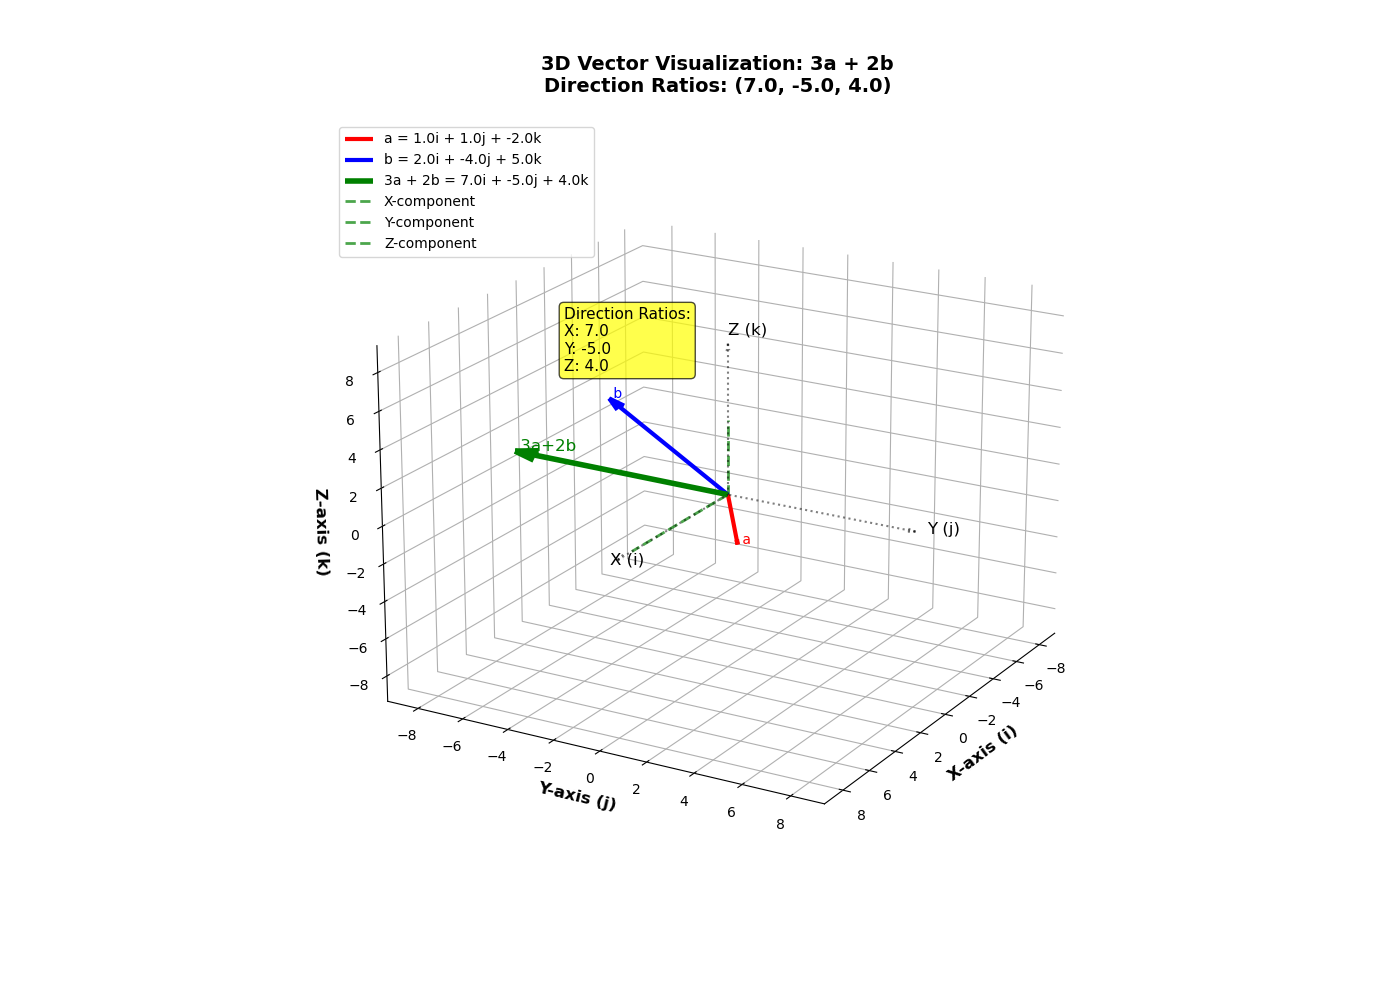
\includegraphics[height=1\textheight, keepaspectratio]{figs/fig1.png}
    \label{figure_1}
\end{figure}
\end{frame}

\end{document}
